\section{Kraftförsörjning}
\textbf{HAREC a.\ref{HAREC.a.3.3}\label{myHAREC.a.3.3}}
\label{kraftaggregat}
\index{kraftförsörjning}
\index{kraftaggregat}

Den elektriska energi, som behövs för elektronikutrustningar, hämtas
från det allmänna elektricitetsnätet, ett batteri eller en
ackumulator. Vissa batterityper kan återuppladdas och kallas då
ackumulator.

Batterier och ackumulatorer avger en nominell spänning, som beror av
de ingående materialen och givetvis av laddningstillståndet. Moderna
utrustningar för amatörradio är utförda för 12~V likström och försörjs
vanligen från ett nätanslutet kraftaggregat. På så sätt kan mobila
radioutrustningar även försörjas från startackumulatorn i fordonet.

Handburna radioutrustningar försörjs från en inbyggd ackumulator, som
laddas från stationär laddare.

Äldre stationära radioutrustningar drivs nästan alltid med nätanslutna
kraftaggregat med en eller flera transformatorer och
likriktare. Alternativt kan samma transformators sekundärsida vara
försedd med flera lindningar för olika spänningar och strömkretsar.

Det allmänna elnätet i Sverige levererar växelspänning med frekvensen
50~Hz. Nätspänningen för hushållsändamål är numera 400/230~V.

Tidigare importerade utrustningar i marknaden kan vara utförda för
andra nätspännings- och skyddsjordningssystem än vad som nu tillämpas
i Sverige. Försiktighet med sådan utrustning rekommenderas.

\subsection{Halv- och helvågslikriktning m.m.}
\textbf{HAREC a.\ref{HAREC.a.3.1.1g}\label{myHAREC.a.3.1.1g}, a.\ref{HAREC.a.3.3.1}\label{myHAREC.a.3.3.1}}
\index{likriktning}
\index{rectifier}

\begin{wrapfigure}{R}{0.5\textwidth}
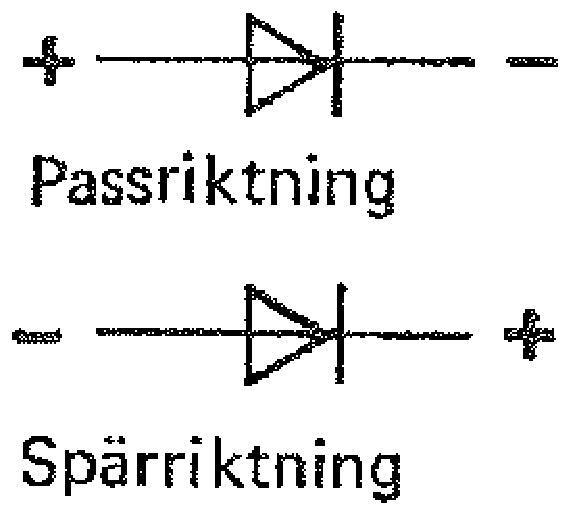
\includegraphics[width=0.5\textwidth]{images/cropped_pdfs/bild_2_3-34.pdf}
\caption{Halvledardioder}
\label{fig:BildII3-34}
\end{wrapfigure}

Bild \ref{fig:BildII3-34}

\emph{Likriktning} (eng. \emph{rectificiation}) av spänningar och strömmar i en
krets görs med ''elektroniska ventiler'', som släpper igenom ström endast i den
s.k. passriktningen och stoppas i spärriktningen. En sådan strömventil
kallas för diod och kan vara av typen vakuumrör eller halvledare. I
moderna konstruktioner används uteslutande halvledardioder i
likriktarkopplingar.

\begin{figure}
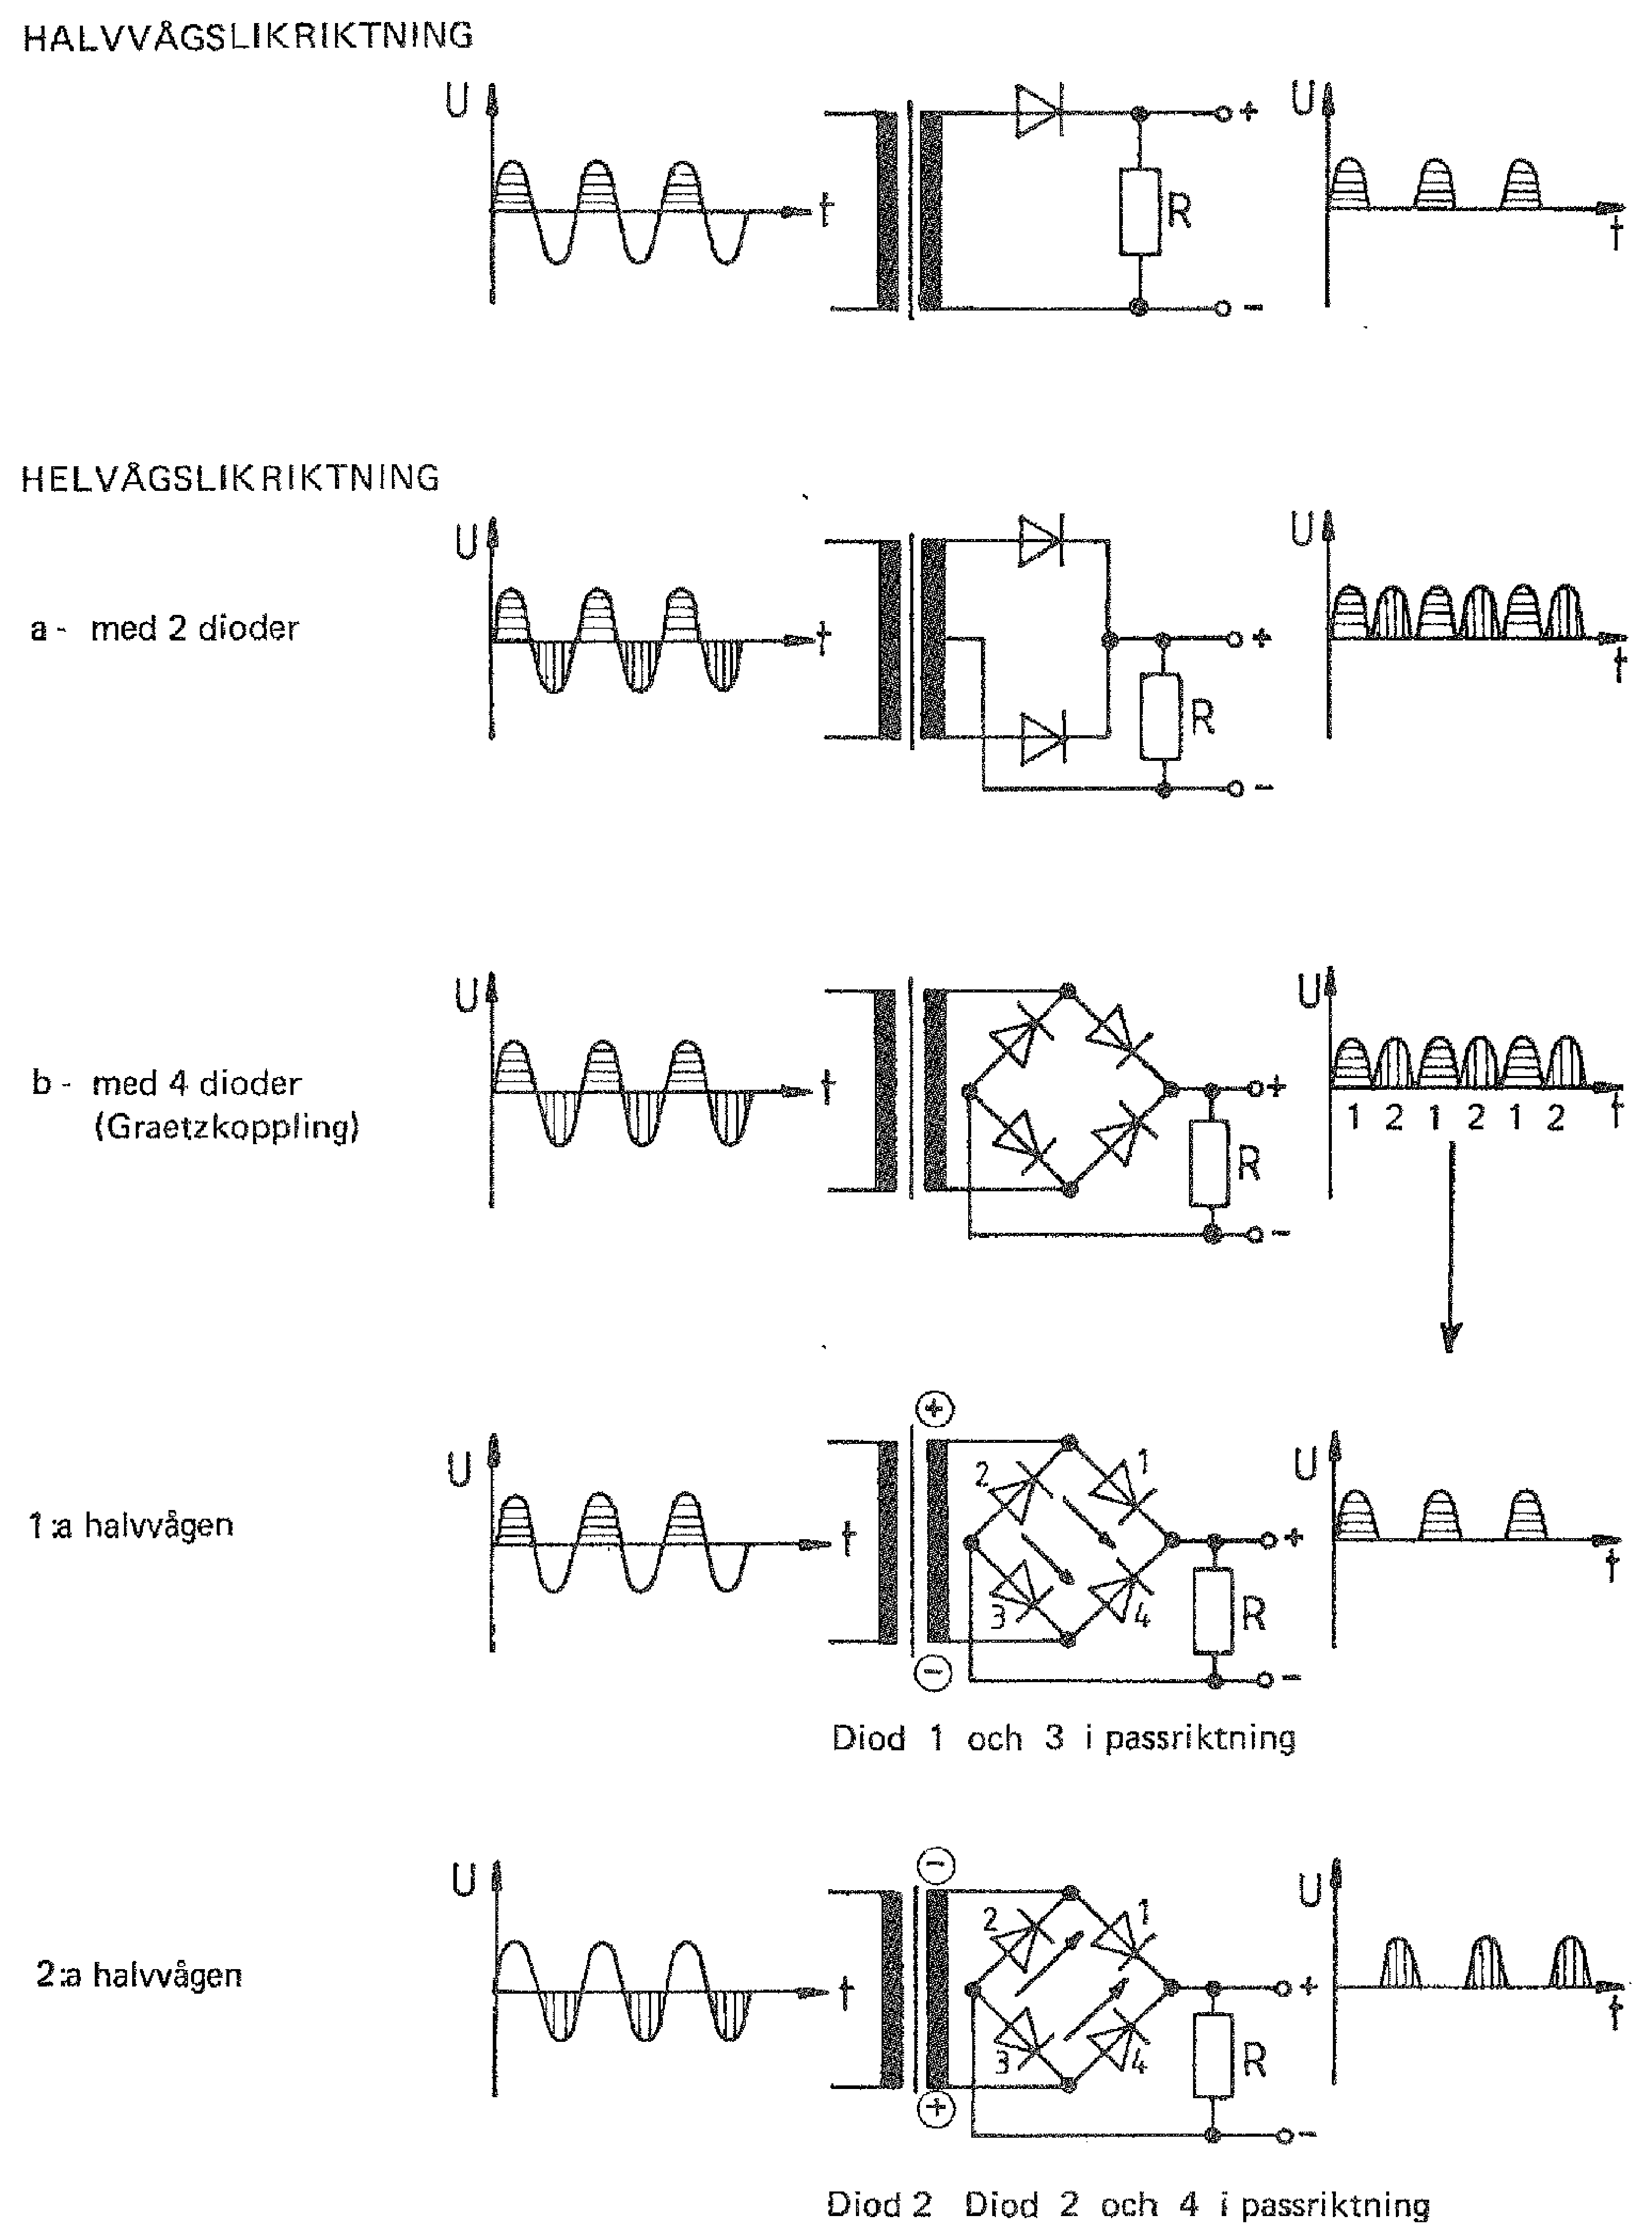
\includegraphics[width=\textwidth]{images/cropped_pdfs/bild_2_3-35.pdf}
\caption{Halv- och helvågslikriktning}
\label{fig:BildII3-35}
\end{figure}

Bild \ref{fig:BildII3-35}

\subsubsection{Halvvågslikriktning}
\index{halvvågslikriktning}
\index{likriktning!halvvågs}

Vid \emph{halvvågslikriktning} (eng. \emph{half wave rectifier}) släpps endast
varannan halvvåg av en växelspänning igenom. I den strömkrets, som bildas av
transformatorns sekundärlindning, dioden och belastningen, flyter därför ström
endast under varannan halvperiod.

\subsubsection{Helvågslikriktning}
\index{helvågslikriktning}
\index{likriktning!helvågs}
\index{Graetz-brygga}

I följande kopplingar med två respektive fyra dioder släpps varje
halvvåg av transformatorns växelspänning igenom så att alla halvvågor
får samma polaritet. Ström flyter genom belastningen i samma riktning
under varje halvperiod. Följande sätt att anordna \emph{helvågslikriktning}
(\emph{full wave rectifier}) är vanliga:
\begin{itemize}
\item Med två dioder och mittuttag på transformatorns
  sekundärlindning. Den ena dioden och ena lindningshalvan släpper
  igenom ström till belastningen under ena halvperioden. Den andra
  dioden och andra lindningshalvan under följande halvperiod o.s.v.

\item Med fyra dioder (s.k. Graetz-brygga) och inget mittuttag på
  transformatorns sekundärlindning, släpper dioderna 1 och 3 igenom
  ström under den ena halvperioden.  Dioderna 2 och 4 släpper igenom
  ström under följande halvperiod o.s.v.
\end{itemize}

\subsection{Glättningskretsar}
\textbf{HAREC a.\ref{HAREC.a.3.3.2}\label{myHAREC.a.3.3.2}}
\index{glättning}
\index{kraftaggregat!glättning}

\begin{figure}
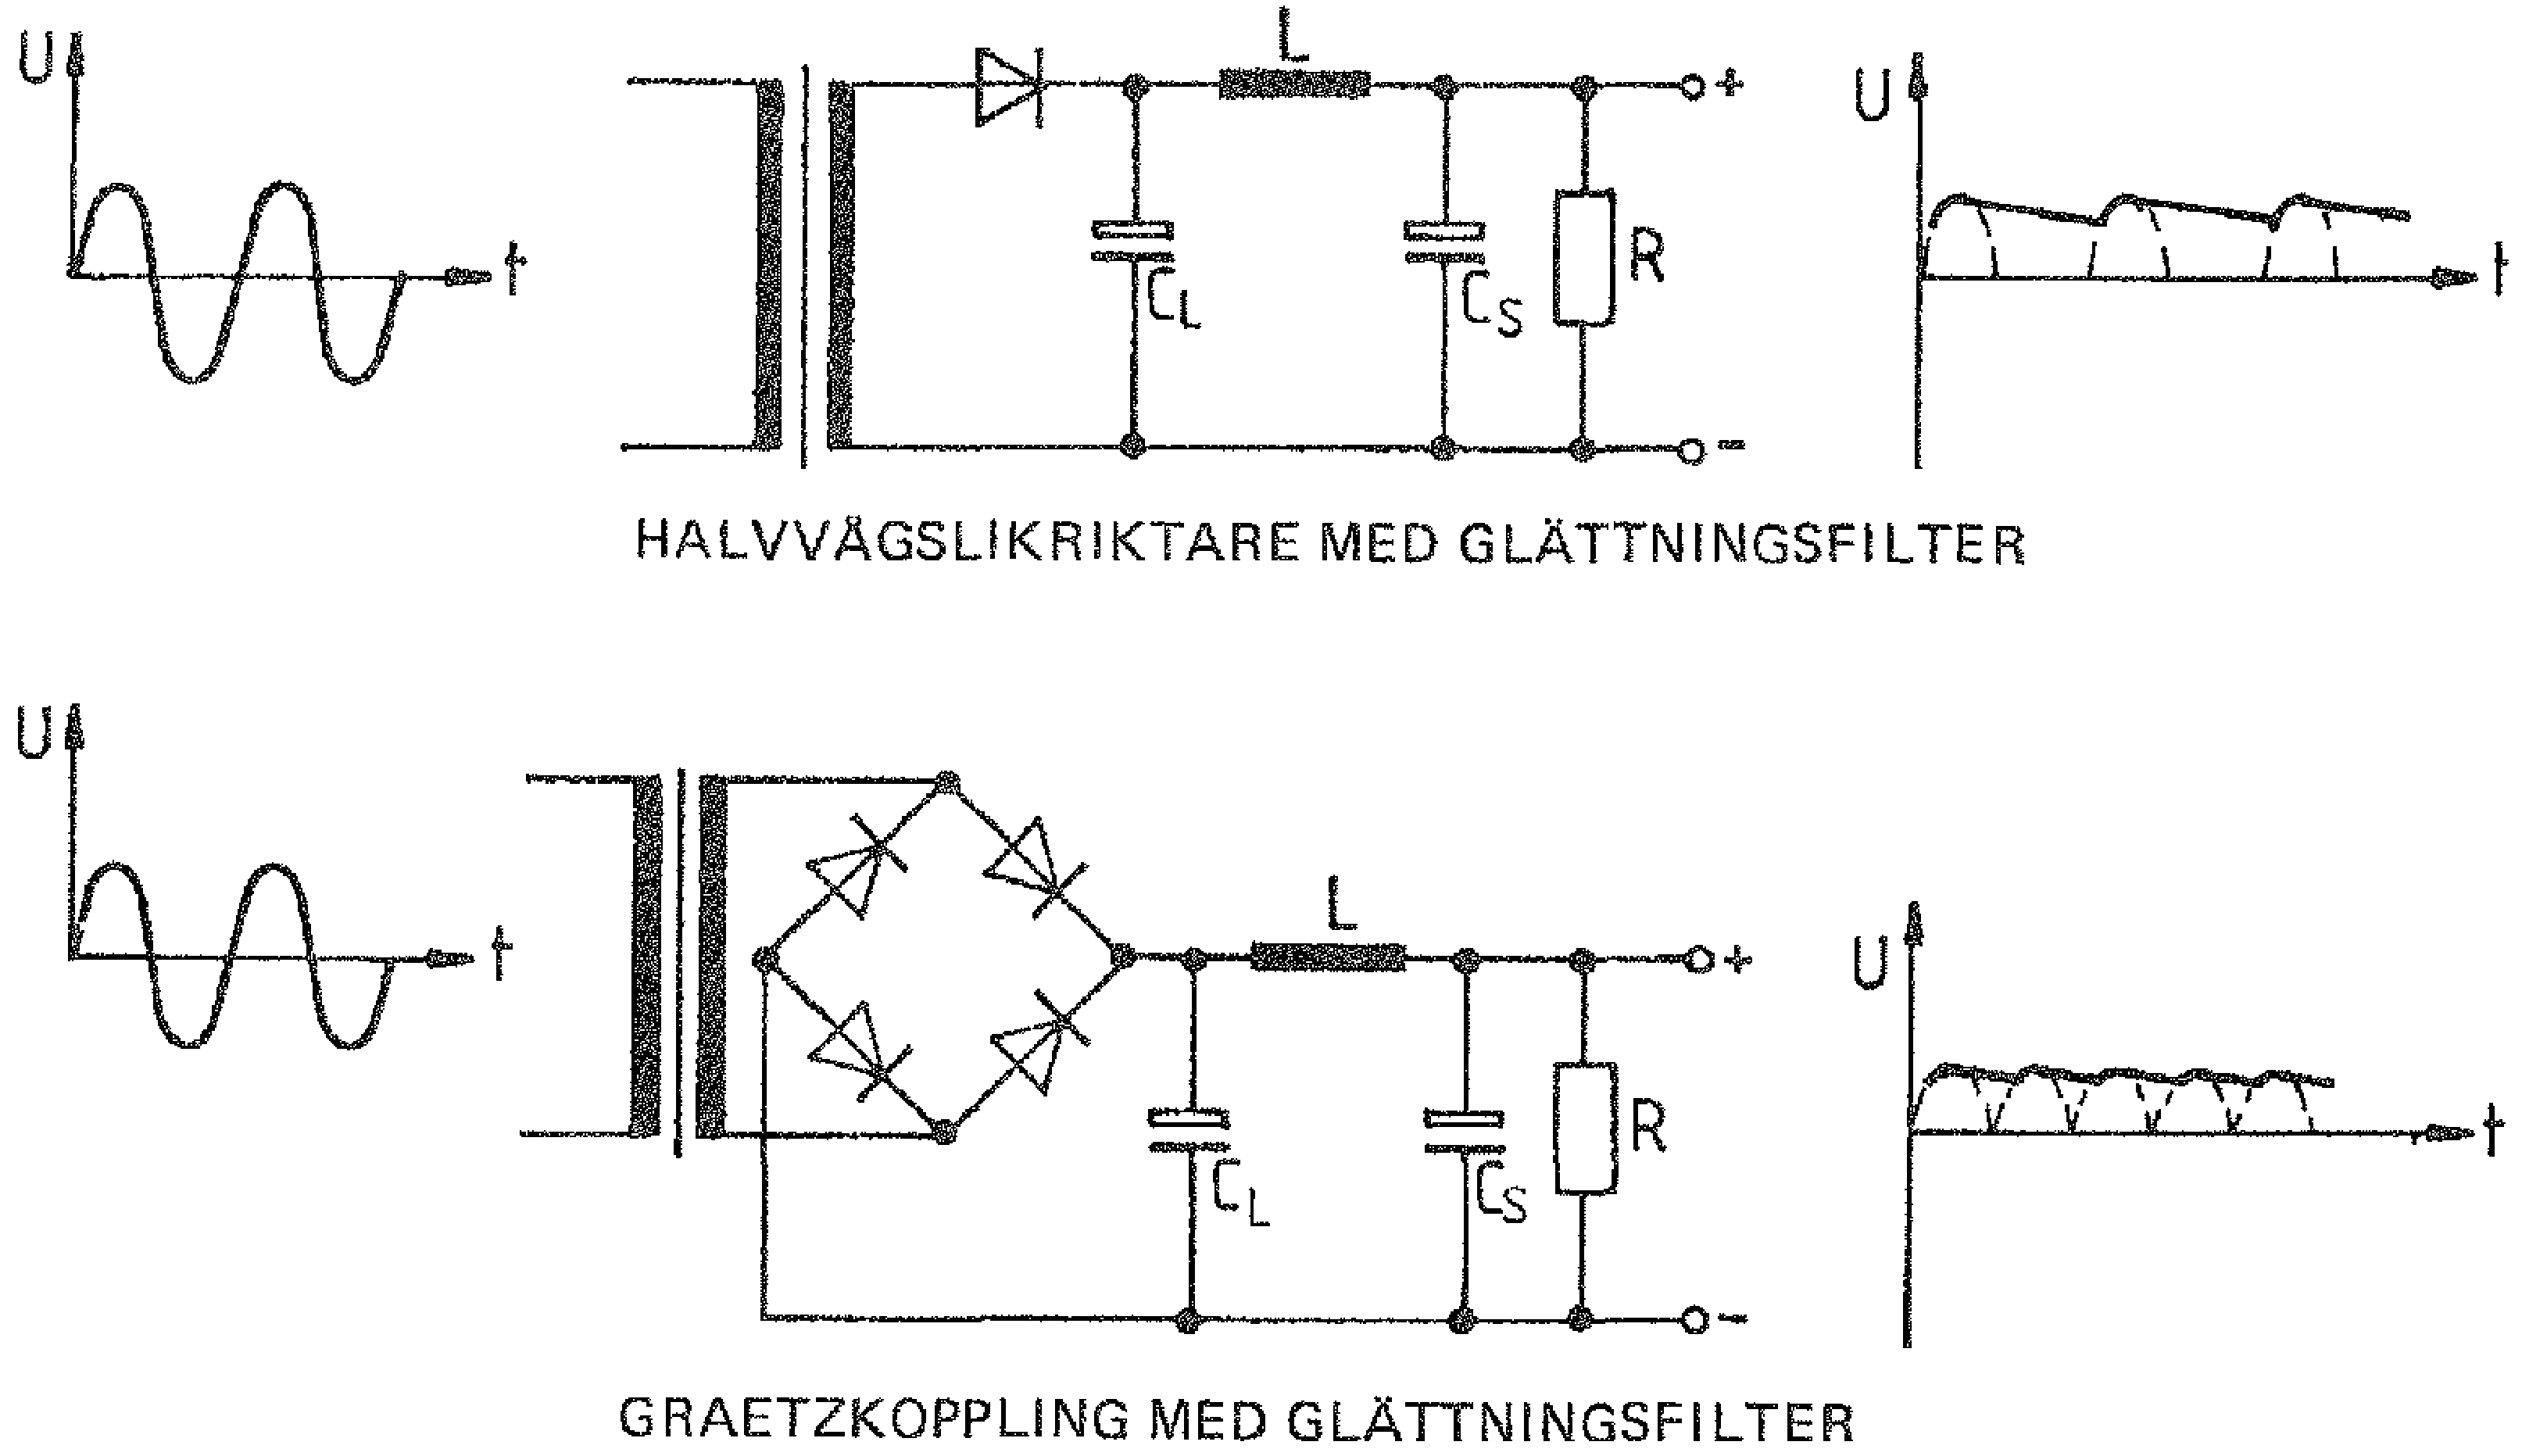
\includegraphics[width=\textwidth]{images/cropped_pdfs/bild_2_3-36.pdf}
\caption{Glättning av likspänning}
\label{fig:BildII3-36}
\end{figure}

Bild \ref{fig:BildII3-36}

Efter likriktningen har växelspänningen omvandlats till en pulserande
likspänning som kan ''glättas''. Efter likriktarna ansluts då ett
glättningsfilter, som t.ex. kan bestå av laddningskondensatorn CL,
induktansen L (s.k. drossel) och glättningskondensatorn C 8.
Parallellt över denna kondensator ligger för elsäkerhetens skull en
urladdningsresistor med hög resistans alltid inkopplad.

Säkerhetsresistorn ska ladda ur kondensatorerna, när kraftaggregatet
inte är anslutet till strömförsörjningen och
belastningen. Säkerhetsresistorn (eng. bleeder) ska vara av
trådlindad typ och kunna tåla fyra gånger sin egen effektförbrukning.

I obelastat tillstånd är spänningen över laddningskondensatorn
\(\sqrt{2}\) större än effektivvärdet på transformatorns
sekundärspänning. När en transformator i tomgång har ett effektivvärde
av 230~V över sekundärlindningen, så blir spänningen över
säkerhetsmotståndet \(230\cdot\sqrt{2} \approx 325\)~V.

\subsubsection{Spänningshöjande likriktarkopplingar}
\index{kraftaggregat!spänningshöjning}
\index{kraftaggregat!spänningsdubbling}

Vid likriktning av växelspänningar enligt någon av ovanstående metoder
behövs en sekundärspänning från transformatorn av minst samma storlek
som den önskade likspänningen. Önskas en högre likspänning, t.ex. den
dubbla, men med samma sekundärspänning på transformatorn, så måste en
speciell likriktarkoppling användas.

\begin{figure}
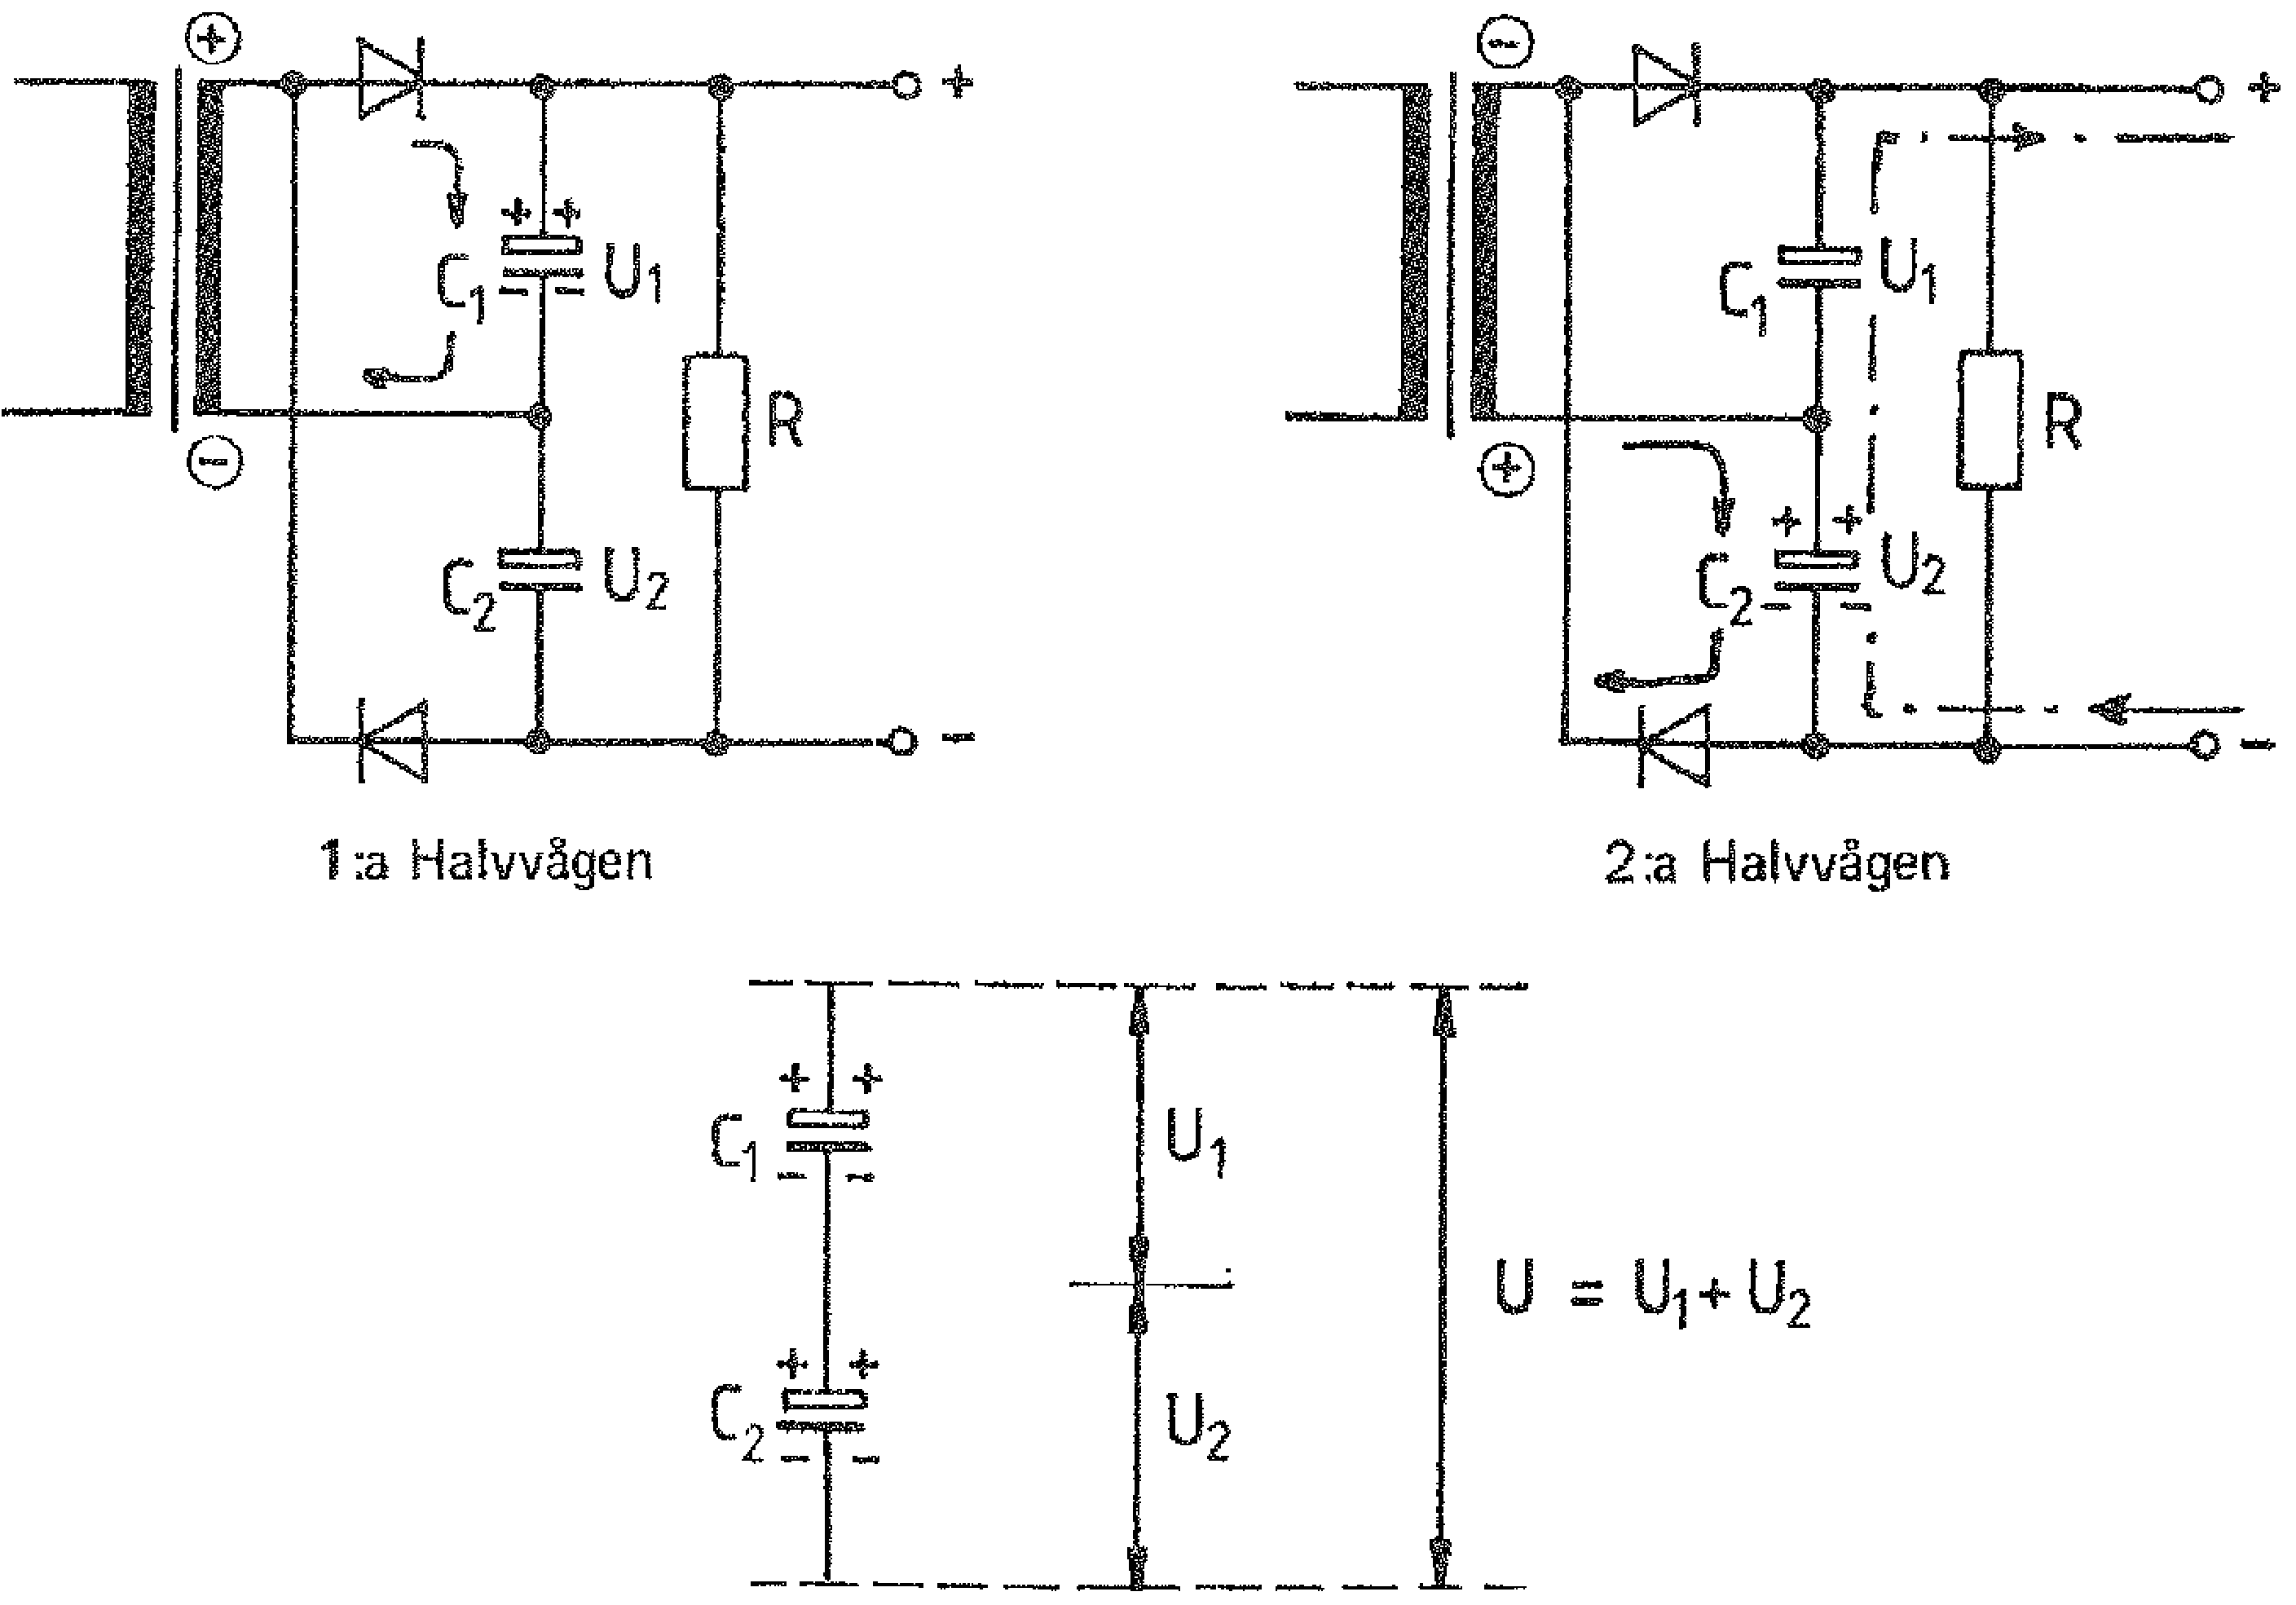
\includegraphics[width=\textwidth]{images/cropped_pdfs/bild_2_3-37.pdf}
\caption{Likriktarkoppling med spänningsdubbling}
\label{fig:BildII3-37}
\end{figure}

Bild \ref{fig:BildII3-37}

Bilden visar en spänningsfördubblande koppling. Under 1:a halvvågen
laddas kondensator \(C_1\) upp. Under 2:a halvvågen laddas kondensator
\(C_2\) upp. Kondensatorerna är kopplade i serie och den ena
kondensatorn hinner inte bli urladdad under tiden som den andra
kondensatorn blir uppladdad. Följden blir att belastningen ser
kondensatorernas spänningar som seriekopplade och därmed har en
spänningsfördubbling erhållits. Det finns även kopplingar för
flerdubbling av spänningar, vilket bl.a. används för att alstra
accelerationsspänningen för TV-bildrör.

\subsection{Spänningsstabilisering}
\textbf{HAREC a.\ref{HAREC.a.3.3.3}\label{myHAREC.a.3.3.3}}
\index{spänningsstabilisering}
\index{kraftaggregat!spänningsstabilisering}

\begin{wrapfigure}{R}{0.5\textwidth}
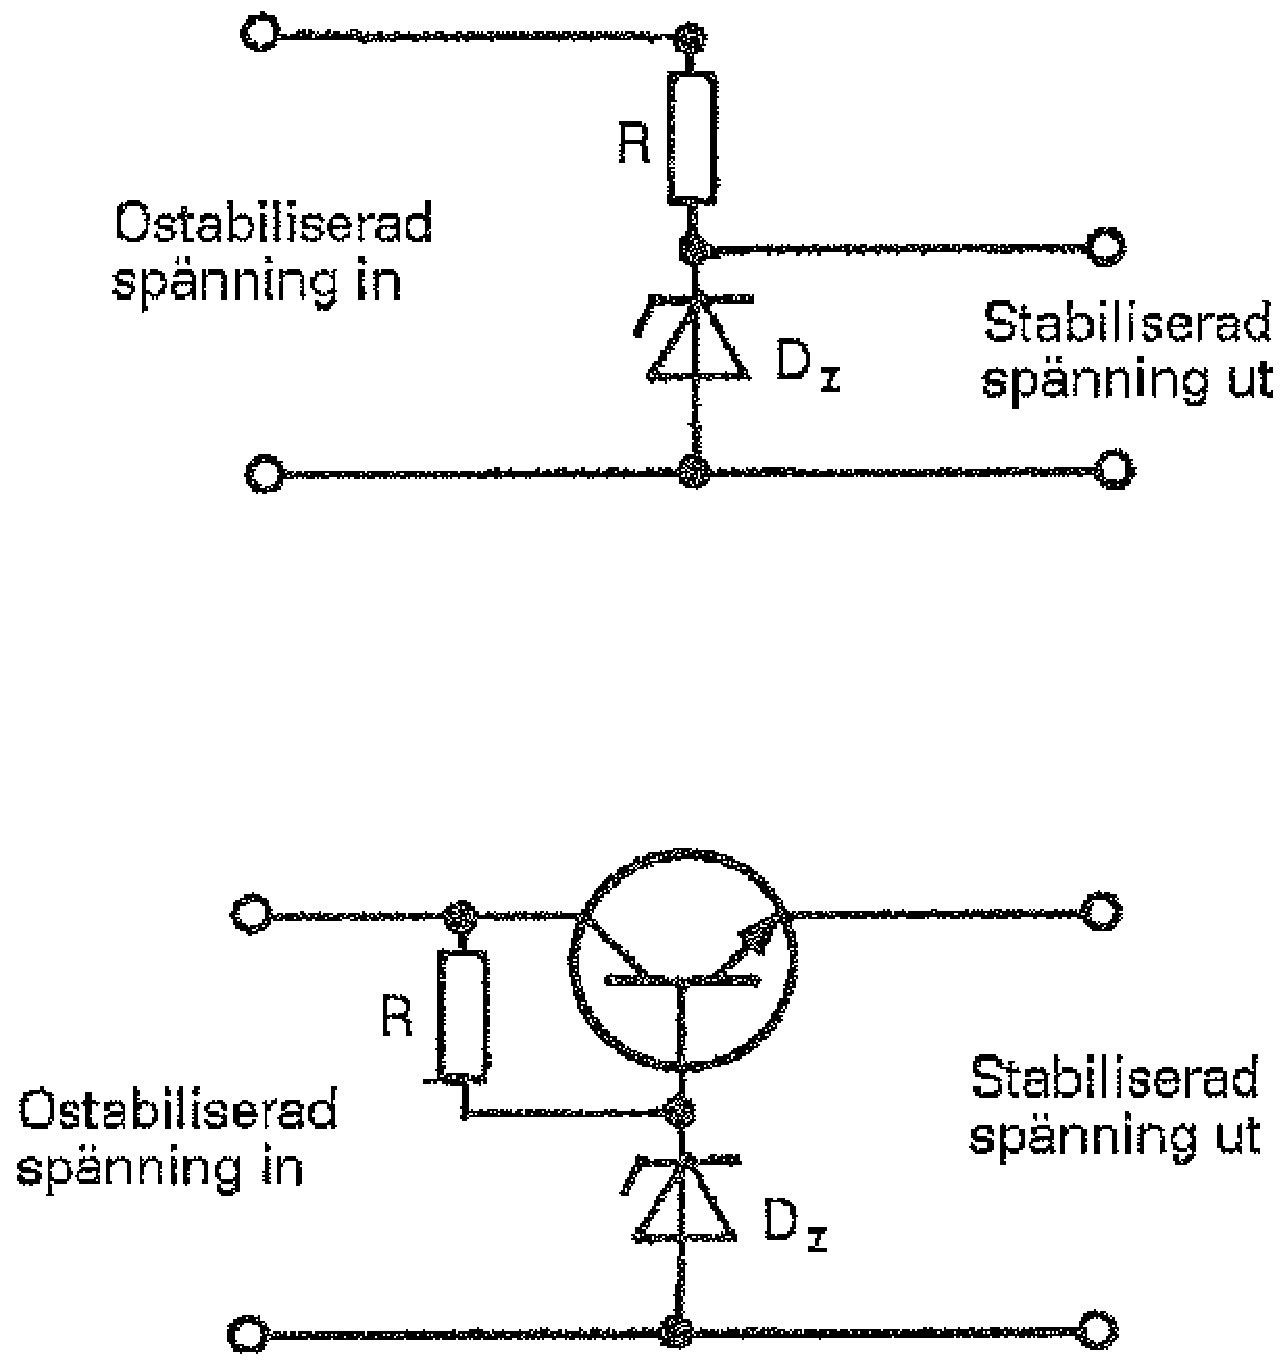
\includegraphics[width=0.5\textwidth]{images/cropped_pdfs/bild_2_3-38.pdf}
\caption{Spänningsstabilisering}
\label{fig:BildII3-38}
\end{wrapfigure}

Bild \ref{fig:BildII3-38}

Utspänningen från ett kraftaggregat tillåts i många fall att endast
variera mellan vissa värden, fastän inspänningen och strömuttaget
varierar mycket. Ett vanligt sätt att hålla konstant spänning är att
anordna en automatisk spänningsdelare efter glättningsfiltret.

Glimlampan och zenerdioden har egenskapen att spänningsfallet över dem
är i det närmaste konstant inom ett visst strömområde. Glimlampor
arbetar på högre spänningar och används i utrustningar med
elektronrör. Zenerdioder arbetar på de lägre spänningar som används i
dagens elektronik.

Stabiliseringen tillgår så att t.ex. zenerdioden får ingå som aktiv
del i en spänningsdelare, som består av en resistor i serie med
belastningen och zenerdioden parallellt med den. Zenerdioden tar upp
variationerna i belastningsströmmen, varvid spänningen över
spänningsdelarens uttag blir stabiliserad. Vid större strömuttag kan
zenerdioden inte ensam ta upp hela den effekt som den reglerar bort. I
stället tas effekten upp av en eller flera transistorer som i sin tur
regleras av zenerdioden.

I vissa fall behövs i stället en reglerad utström från kraftaggregatet
Även för detta ändamål används kopplingar med zenerdioder och
transistorer.

\subsection{Switchaggregat}
\textbf{HAREC a.\ref{HAREC.a.3.3.4}\label{myHAREC.a.3.3.4}}
\index{switchaggregat}
\index{kraftaggregat!switchaggregat}

Senare utvecklingsformer är s.k. switchade aggregat. I sådana regleras
spänningen eller strömmen genom sönderhackning (switching). Genom att
förändra förhållandet mellan till- och frånslagstiderna kan man skapa
det önskade medelvärdet. Metoden ger hög verkningsgrad.
Switch-frekvensen är i storleksordningen 20~kHz eller högre.
På grund av den högre frekvensen krävs mindre kondensatorer i
switchade aggregat. Sådana kraftaggregat kan emellertid ge störningar,
varför effektiv avstörning behövs.

Kraftaggregat som omvandlar från nätspänning till likspänning använder
den primär-switchade principen. I ett primär-switchat aggregat likriktas
nätspänningen innan den switchas på primärspolen i transformatorn.
Eftersom frekvensen är relativt hög, behöver transformatorns kärna inte
vara så stor, eftersom lägsta frekvensen inte riskerar mätta den på samma
sätt som vid nätfrekvensen (50~Hz). På sekundärsidan likriktas sedan
spänningen och glättning kan ske med relativt små kondensatorer på grund
av den höga frekvensen. Genom att återmata spänningen till primärsidan, kan
utspänningen regleras i primär-switchningen istället för att behöva
stabilisera spänningen på sekundärsidan, vilket skulle leda till ytterligare
förluster som därigenom kan undvikas. Ett primärswitchat aggregat ska ha
nätfilter för att klara EMC-krav, något som även är till nytta att hålla
störningar nere.

En annan kategori av switchade aggregat är det som finns för
likströmsomvandling, även känt som DCDC-omvandling. Dessa har inte alltid
galvanisk isolation mellan in och utgång, men de kan vara värdefulla
kompletteringar, genom den enkelhet de har. Det har även kommit switchade
ersättare med lägre effektförlust än i de traditionella linjära regulatorerna i
78 och 79 serien.
Problemet med dessa är att de kan producera störningar om man
inte tar hänsyn till det. Detta är ett exempel på en enklare så kallad
drop-omvandlare som kan sänka spänningen med switchning. Andra omvandlare kan
höja spänningen eller byta polaritet på den. Dessa omvandlare har inte sällan
frekvenser på 200~kHz till 2~MHz idag.

Switchade kraftaggregat och spänningsstabiliseringar är nu en naturlig del
av elektroniken, då effektförlusterna kan hållas mycket lägre än gamla
linjära aggregat. Switchingen innebär dock att det kan läcka ut störningar
både på ingång och utgång så väl som direkt från själva aggregatet i sig.
En del tillåter manuell styrning av switch-frekvensen, varvid man kan flytta
störningarna till en frekvens där deras påverkan minskar. Störningarna kan vara
både i differentiell och gemensam mod, och därför bör man vara uppmärksam på det när
man försöker göra avstörning. Lyckligtvis är switch-frekvenserna relativt höga,
vilket förenklar komponentval.
